\documentclass[a4paper,oneside,12pt]{report}

%%%%%%%%%%%%%%%%%%% LOAD PACKAGES %%%%%%%%%%%%%%%%%%%%%
%Get support for äöüßÄÖÜ
\usepackage[utf8]{inputenc}
%Get support for word separation
\usepackage[T1]{fontenc}
%Direkte Verwendung von Umlauten
\usepackage[ansinew]{luainputenc}
%Get Support for US english and german
\usepackage[english,ngerman]{babel}
%verbesserter Randausgleich
\usepackage{microtype}
%zulässiger Wortzwischenraum erhöhen für noch besseren Randausgleich und Blocksatzbildung
\setlength\emergencystretch{1em}
%Einrücken nach Absatz für gesamtes Dokument abstellen
\setlength{\parindent}{0pt} 
%Bildbeschreibung zentrieren
\usepackage[center]{caption}
%Support for Graphics .png .jpg .pdf 
\usepackage{graphicx}
%Zusätzliche Option[H] bei Bildern - Hier und und sonst nirgends!
\usepackage{float}
%Adjust the page margins asymmetrical, Need to be before subfig
\usepackage[left=3cm, right=2.5cm, top=3cm, bottom=3cm, a4paper, portrait]{geometry}
%Kopf- und Fußzeilen
\usepackage{fancyhdr}
%für Fußnote (linksbündig)
\usepackage[flushmargin,bottom]{footmisc}
%Erweiterung des Mathematikmoduses
\usepackage{amsmath}
%Use Palatino Linotype 
\usepackage{mathpazo}
%Don´t show "Kapitel 1" at \chapter
\usepackage{titlesec} 
\titleformat{\chapter}{\bfseries\Huge}{\thechapter\quad}{0em}{}
%Abstand Kapitelüberschiften zum Kopfrand
\titlespacing{\chapter}{0pt}{*-2}{*1.5}
\usepackage{setspace}
\AtBeginDocument{\renewcommand{\chaptername}{}}
%Tabellenspalten/zeilen einfärben
\usepackage{colortbl}
%variable Tabellenbreite
\usepackage{tabularx}
%Multirow in Tabelle
\usepackage{multirow}
%Tabellenüberschrift links oben!
\usepackage[singlelinecheck=false]{caption}
%Programmcode einfügen
\usepackage{listings}
%Programmcode Farben ändern
\usepackage{xcolor}
%Hyperlink
\usepackage[colorlinks=true,linkcolor=black, citecolor=black, urlcolor=black]{hyperref}
%Ordnerstruktur erstellen
\usepackage{dirtree}
\usepackage{subfigure}
%Abkuerzungen
\usepackage{acronym}
%Highlighting
\usepackage{color,soul}
%Unterstützung für textumflossenes Bild 
\usepackage{wrapfig}


%//%%%%%%%%%%%%%%%%%% END LOAD PACKAGES %%%%%%%%%%%%%%%%%%%%
%//%%%%%%%%%%%%%%%%%% SETTINGS %%%%%%%%%%%%%%%%%%%%%%%%%
%Adjust headings and footers --> \usepackage{fancyhdr}
%Give the headings some space
\setlength{\headheight}{20pt}
%This is valid for all pages exept chapters
\pagestyle{fancy}

\fancyhf{} % clear all headers and footers
%Ausrichtung Kopf- /Fußzeile
\lhead[]{\fancyplain{}{\leftmark}}
\cfoot[]{\thepage}
\renewcommand{\headrulewidth}{0.4pt}
%For \chapters \maketitle
\fancypagestyle{plain}{%
	\fancyhf{} % clear all header and footer fields
	\cfoot[]{\thepage}%
	\renewcommand{\headrulewidth}{0pt}
	\renewcommand{\footrulewidth}{0pt}
}
%Deactivate command --> small letter
\let\MakeUppercase\relax
%Tiefe von Inhaltsverzeichnis 
\setcounter{secnumdepth}{3}
\setcounter{tocdepth}{3}
%Programmcodeeinstellungen
\lstset{
	backgroundcolor=\color{black!5},
	tabsize=4,
	language=C++,
	captionpos=b,
	tabsize=3,
	frame=lines,
	numbers=left,
	numberstyle=\scriptsize,
	numbersep=5pt,
	breaklines=true,
	showstringspaces=false,
	basicstyle=\scriptsize,
	%identifierstyle=\color{magenta},
	keywordstyle=\color[rgb]{0.8,0.4,0},
	commentstyle=\color[rgb]{0.9,0.3,0.9,},
	stringstyle=\color{green},
	emphstyle=\color{blue},
}
%Programmcodeeinstellungen, style Arduino
	\lstdefinestyle{Arduino}{%
		%style=numbers,
		keywords={soup},%                 define keywords
		%morestring=[s]{<}{>},%			  define <> as strings
		morecomment=[l]{\#},%             treat // as comments
		morecomment=[s]{/*}{*/},%         define /* ... */ comments
		emph={void, for, else, if, in, HIGH, OUTPUT, LOW, int, uint8_t, self, def, True, False, print, from, import, as, class, try, except, not, or, return, global},%        keywords to emphasize	
}


%Bennenung von Caption bei Programmcode 
	\renewcommand{\lstlistingname}{Programmcode}
	\renewcommand{\lstlistlistingname}{\lstlistingname}
	%Bennenung von Bilderquelle als "Quelle:"
	\newcommand*{\quelle}{%
		\footnotesize Quelle:
	}

%//%%%%%%%%%%%%%%%%%% END SETTINGS %%%%%%%%%%%%%%%%%%%%%%%%%

%\\%%%%%%%%%%%%%%%%%% DOCUMENT %%%%%%%%%%%%%%%%%%%%%%%%%


\begin{document}
	%%%%Bearbeitet
%Deckblatt
\thispagestyle{empty}
\begin{center}
	
\includegraphics[scale=0.5]{Bilder/HM1_logo.png}


	
	\vspace{1.5cm}
	\huge{Programmcode}\\\vspace{1.5cm}
	\large{im Zusammenhang mit der Bachelorarbeit}\\\vspace{0.5cm}
	\large{an der}\\\vspace{0.5cm}
	
	\huge{Hochschule München}\\
	\normalsize {für angewandte Wissenschaften}\\\vspace{0.5cm}
	\large{mit dem Titel}\\\vspace{1cm}
    \begin{center}
		\Huge{\textbf{Aufbau eines automatischen Testers für ein automotive Messtechnik Rack}}\\[2.0cm]
    \end{center}
    
	
	
	\large{Fakultät für Informatik und Mathematik}\\
	\normalsize {Studiengang Master Wirtschaftsinformatik}\\\vspace{2.1cm}
	
\end{center}

	
\newpage
\thispagestyle{empty}
\begin{flushleft}	
	\begin{tabular}[H]{ll}
		
		Ersteller: & \large{Johannes Knippel, Anja Wolf,}\\[0.2cm]
		 			& \large{Johanna Sickendiek, Skanny}\\[0,2cm]
		1. Prüfer:		  & \large{blablablabla}\\[0.2cm]
		2. Prüfer:		  & \large{loablebli}\\[.7cm]
		
		
		Betreuer an der Hochschule München: 	& \large{Prof. Dr. Rainer Schmidt}\\[0.5cm]
		Ausgabedatum:					& \large{19.03.2018}\\[0.5cm]
		Abgabedatum:					& \large{22.07.2018}\\[3.5cm]
	
		
		%FeldLinks für OrtDatum1	
		%\hspace*{\fill}
	
		\parbox{7cm}{\hrule\medskip Ort, Datum\\ [0.3cm]}	&	\parbox{7cm}{\hrule\medskip Unterschrift des 1. Prüfers\\ [0.2cm]Blaaaaaaaaaaaabla}\\[1.5cm]
		\parbox{7cm}{\hrule\medskip Ort, Datum\\ [0.31cm]}	&	\parbox{7cm}{\hrule\medskip Unterschrift des 2. Prüfers\\ [0.2cm]Blaaaaaaaaaaaabla}\\[1.5cm]
		\parbox{7cm}{\hrule\medskip Ort, Datum\\ [0.33cm]}	&	\parbox{7cm}{\hrule\medskip Unterschrift des Verfassers\\ [0.2cm]Johannes Knippel}\\[1.5cm]
		\parbox{7cm}{\hrule\medskip Ort, Datum\\ [0.33cm]}	&	\parbox{7cm}{\hrule\medskip Unterschrift des Verfassers\\ [0.2cm]Anja Wolf}\\[1.5cm]
		\parbox{7cm}{\hrule\medskip Ort, Datum\\ [0.33cm]}	&	\parbox{7cm}{\hrule\medskip Unterschrift des Verfassers\\ [0.2cm]Johanna Sickendiek}\\[1.5cm]
		\parbox{7cm}{\hrule\medskip Ort, Datum\\ [0.33cm]}	&	\parbox{7cm}{\hrule\medskip Unterschrift des Verfassers\\ [0.2cm]Skanny}\\
	\end{tabular}
\end{flushleft}

	
	
	

	\pagenumbering{Roman}


%												 Inhaltsverzeichnis
	\newpage
	\tableofcontents
	
	
	
	
	
%											    Kapitel 1 - Einleitung
	%\newpage
	\pagenumbering{arabic}
	\setstretch{1.5}
	\chapter{Problemstellung}\label{probstellung}
	
		Für nahezu Jedermann bietet das WWW im Vergleich zu damaligen Zeiten ungeahnte Möglichkeiten der Recherche und Themenfindung. Noch nie waren so viele Informationen öffentlich einsehbar wie heute. Meist sind jedoch die gewünschten Inhalte an vielen unterschiedlichen Orten im Web verteilt, auf unterschiedlichste Weisen formatiert oder aufgrund schlechter Informationsarchitektur nur mit größerem Aufwand zu erreichen. Grundsätzlich kann die Fülle an Ergebnissen überfordern und nicht immer sind alle relevanten Inhalte über gängige Suchmaschinen auffindbar. Das bedeutet dann oft die mühsame Suche nach den relevanten Informationen in nicht immer nutzerfreundlich gestalteten Datenbanken. Bei so gut wie allen Recherchearbeiten besteht die Aufgabe heutzutage darin, die sprichwörtliche „Nadel im Heuhaufen“ zu finden. In vielen Fällen wünscht man sich einen gewissen Grad an Automatisierung. Daher soll im Rahmen eines Forschungsprojektes an der Hochschule München ein Tool entworfen werden, das Informationen und Inhalte von Webseiten automatisiert gewinnt. 
		\\
		Programmiertechnisch bedient man sich hierfür meistens vorhandener Schnittstellen, die die jeweiligen Quellen zur Verfügung stellen. Neben anwendungsspezifischen APIs sind dies zum Beispiel RSS- oder AtomFeeds, die in eigene Datenbanken geladen und von dort aus weiterverarbeitet werden können. \cite{bib-atomfeed} Die Informationen liegen in diesen Fällen also bereits in einem strukturierten Format vor und enthalten wenig bis gar keinen überflüssigen Inhalt.
		\\
		Hingegen wenn keine der genannten Schnittstellen angeboten werden, bleibt die ständige Beobachtung dieser Inhalte schwierig. Sofern es sich bei den Quellen um einfach strukturierte HTML-Seiten handelt, kann man sich mit verschiedenen Tools weiterhelfen. Gerade bei öffentlichen Datenbanken, deren Inhalte über Webformulare abgefragt werden („Deep Web“), ist dies jedoch meistens nicht möglich. \cite{bib-deepweb} Hier können Webscraper weiterhelfen, die das automatisierte „Auslesen“ von bestimmten strukturierten	oder semi-strukturierten Inhalten aus öffentlich zugänglichen Webseiten ermöglichen. 
		\\
		\newline
		Diese Studienarbeit beleuchtet am Beispiel von TripAdvisor wie ein solcher Webscraper implementiert werden kann. Des Weiteren umfasst diese Studienarbeit das automatisierte Abspeichern der gewonnenen Daten in einer strukturierten Datenbank.
		
		%Gewonnene Daten können so Aufschluss über Verhaltensweisen, Interessen und auch mögliche Kaufanregungen geben.
	
	


	\chapter{Grundlagen}\label{grlagen}
	
		\section{Was ist WebCrawling?}
	
			\subsection{Definition, Erläuterung etc.}
	
			\subsection{Wie funktioniert es? (Allgemeine Beschreibung)}
	
			\subsection{Datenstrukturen}
			
				Sowohl der Kontext von Daten, als auch ihre Eigenschaften führen zur Strukturierung dieser in verschiedene Datenarten. Kontextinformationen machen genauere Angaben zu Prozessen in denen die Daten benötigt werden. Eigenschaften hingegen unterscheiden Daten nach Format, Inhalt, Stabilität, Verarbeitung oder Struktur.\\
				Besonders relevant für dieses Projekt ist folglich letzteres – die Struktur von Daten. Hier unterscheidet man grundsätzlich zwischen drei verschiedenen Fällen, strukturierten, semistrukturierten und unstrukturierten Daten.
				\\
				Bei strukturierten Daten sind Metadaten, d.h. strukturgebende Informationen zu Daten vorhanden. Diese können u.a. Auskunft zu Format, erlaubten Werten oder semantischer Bedeutung geben. Ein klassisches Beispiel für strukturierte Daten sind alle möglichen Formen von Datenbanken. Hier müssen zunächst das Schema der Datenbank und deren einzelnen Tabellen festgelegt werden bevor Daten in die definierten Felder einfügt werden können. Somit ist eine einfache Analyse dieser zu einem späteren Zeitpunkt sichergestellt.
				\\
				Bei semistrukturierte Daten sind einzelne Bestandteile strukturiert, es mangelt jedoch an einer eindeutigen strukturierten Gesamtheit. Die Daten sind keinem objektorientierten oder relationalem Datenbankschema untergeordnet.
				\\
				Bei unstrukturierten Daten wird keinem eindeutigen Schema gefolgt, nur einer reinen Bitfolge. Das bedeutet jedoch nicht, dass die Daten gar keine Struktur aufweisen. Diese ist jedoch nicht direkt bzw. eindeutig für den Nutzer erkennbar. Neben Multimedia Daten (Bilder, Musik) finden sich unstrukturierten Daten auch meist in Emails, auf Internetseiten oder in Text-Dokumenten \cite{bib-daten}.
				\\
				\\
				Web Crawling bzw. Web Scraping fokussiert sich daher auf die Transformation von unstrukturierten Daten im Web zu Daten mit strukturgebenden Metadaten. Die gewünschten Informationen werden dabei als unstrukturierte Rohdaten extrahiert und in einer leicht lesbaren und skalierbaren, d.h. strukturierten Form in Listen, Tabellen oder Datenbanken gespeichert (vgl. Abbildung \ref{pic-webcrawler}). Vorteilhaft ist, dass Web Scraping selektiv arbeitet, d.h. lediglich die Daten transformiert für die man sich im Vorfeld entschieden hat. Dies erleichtert eine Analyse der Daten erheblich. Aktuelle Softwares und Tools sind in der Lage, komplette Websites in strukturierte Daten umzuwandeln um diese weiter zu verarbeiten.
				
				\begin{figure}[H]
					\centering
					\begin{minipage}[b]{0.9\textwidth}
						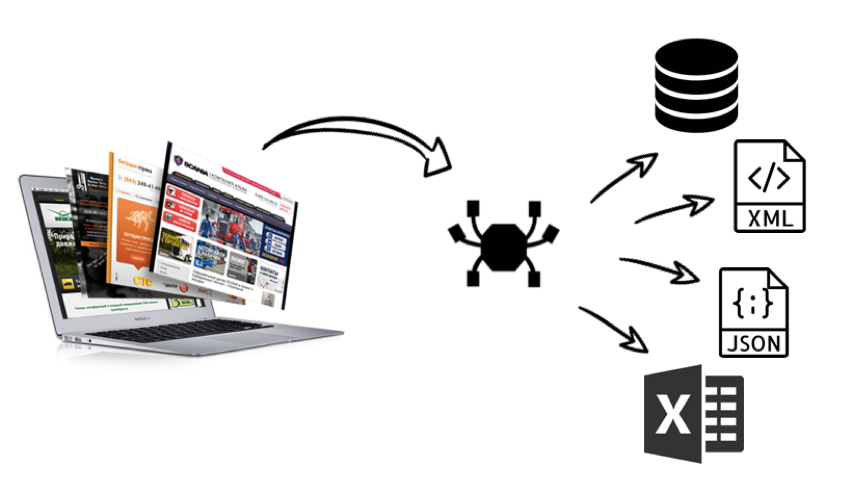
\includegraphics[width=\textwidth]{Bilder/Webcrawler.png}
					\end{minipage}
					\centering
					\caption[Funktionsweise eines Webcrawlers]{Funktionsweise eines Webcrawlers}
					\label{pic-webcrawler}
				\end{figure}
	
		\section{Tripadvisor}
	
			\subsection{Was ist das für eine Webseite? Kurze Beschreibung}
	
	
	
	
	\chapter{Anforderungen}	
	
		\section{Tabelle: Daten TripAdvisor (Welche Daten holen wir uns? Hotel und Restaurants?) details}
	
		\section{Nicht funktionale Anforderungen: Benutzerfreundlichkeit etc.}
	
		bliblablablablubulskjfvba
		öajsvaölfkvpaijsdv
		\\
		öjydfpvoijaf
		v\\jdofhvöankfv
		aposdfjhvpuaohöjvhb
	
	
	
	\chapter{Implementierung}
	
		\section{Konfiguration}
	
			\subsection{Welche Version von Python}
	
			\subsection{Welche Pakete wurden importiert und warum}
	
		\section{BeautifulSoup}
		
			Für die Programmierung des Webcrawlers um Daten von auf TripAdvisor gelisteten Hotels und Restaurants zu scrapen wurde die Python Library ‘BeautifulSoup‘ (\textit{bs4}) verwendet.
			\\
			\newline
			Hierbei handelt es sich um eine Library für XML und HTML parsing, die zunächst als zusätzliches Paket installiert werden muss. Beim Parsen werden XML oder HTML Dateien analysiert und auf ihre einzelnen Bestandteile geprüft. So können jegliche Informationen aus diesen Dateien gesucht bzw. extrahiert werden, vorausgesetzt es sind entsprechende Tags bzw. Attributnamen vorhanden. Ohne diese kann nicht gesucht werden \cite{bib-webpython}. Diese Einfachheit und gleichzeitig große Effizienz sind der westenliche Vorteil, warum das Projekt-Team sich für die Library BeautifulSoup und deren Methoden entschieden hat.
			\\
			\newline
			Um das wahrscheinlich am meisten verwendeten Objekt der BeautifulSoup Library – das BeautifulSoup Object – zu initialisieren, muss diesem ein XML bzw. HTML Dokument oder, wie in unserem Fall, der zu parsenden HTML-Code übergeben werden. BeautifulSoup kann eine URL also nicht selbstständig aufrufen, sondern erst mit dem gespeicherten Quelltext der HTML-Seite arbeiten \cite{bib-bs4}. In unserem Fall wird die TripAdvisor URL des gewünschten Hotels bzw. Restaurants daher zunächst mit einer Methode der Python Library \textit{‘request'} aufgerufen. Diese sendet einen HTTP/1.1 request und pingt die Website an, dass Informationen extrahiert werden möchten. Sobald der Webserver eine \textit{response} sendet wird der Inhalt der URL, d.h. der HTML-Code in einer einfachen String Variable gespeichert. Erst jetzt kann ein neues BeautifulSoup Object initialisiert werden (vgl. Programmcode 4.1).
			\\ 
			\begin{lstlisting} [caption={Initialisierung BeautifulSoup Object}\label{initbs4}, captionpos=b, style=Arduino]
			def get_single_data(self,url):
			source_code = requests.get(url)
			plain_text = source_code.text
			soup = BeautifulSoup(plain_text, "html.parser")
			\end{lstlisting}
			
			Dieses transformiert den komplexen HTML-Code in einen ebenfalls komplexen Baum mit Python Objekten. Die HTML-Tags korrespondieren mit den neuen Tag Objekten des BeautifulSoup Objects \cite{bib-bs4}. Am folgenden Beispiel kann die Struktur eines solchen beispielhaft veranschaulicht werden.
			
			
			\begin{figure}[H]
				\centering
				\begin{minipage}[b]{0.9\textwidth}
					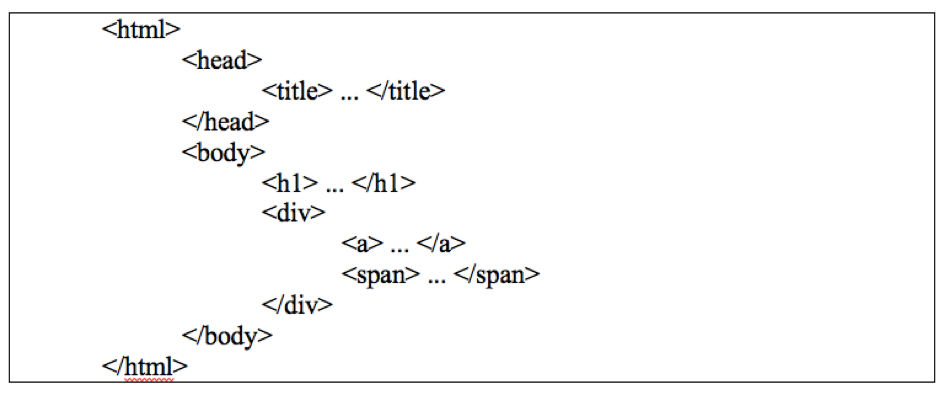
\includegraphics[width=\textwidth]{Bilder/HTMLcode.png}
				\end{minipage}
				\centering
				\caption[HTML Code bs4]{Baum mit Python Objekten \cite{bib-webpython}}
				\label{pic-HTMLcode}
			\end{figure}
			
			Natürlich enthält dieser normalerweise eine weitaus größere Anzahl an Vererbungen, d.h. ineinander verschachtelten Tags, und ist daher komplizierter zu lesen. Jedoch wird anhand dieses Beispiels bereits deutlich, wie die im folgenden beschriebenen Methoden der BeautifulSoup Library damit arbeiten können.
			\\
			\newline
			Sobald das BeautifulSoup Object vorliegt, können die vorhandenen Methoden der bs4 Library genutzt werden. In folgender Tabelle sind die beiden bekanntesten und auch im Programm-Code am meisten genutzten Methoden aufgelistet \cite{bib-bs4}.
		
			\begin{figure}[H]
				\centering
				\begin{minipage}[b]{0.9\textwidth}
					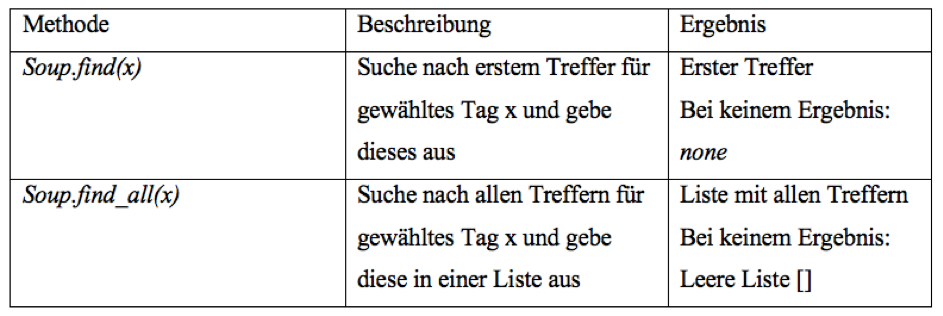
\includegraphics[width=\textwidth]{Bilder/SoupMethoden.png}
				\end{minipage}
				\centering
				\caption[Methoden bs4]{Such-Methoden der Python Library BeautifulSoup \cite{bib-bs4}}
				\label{pic-SoupMethoden}
			\end{figure}
			
			Im folgenden Kapitel werden diese genutzt um den Webcrawler für TripAdvisor erfolgreich zu implementieren.
	
	
		\section{Implementierung WebCrawler}
	
	
			\subsection{Initialisierung BeautifulSoup}
			
				Zunächst wird die URL des gewünschte Restaurants oder Hotels, für welches Daten extrahiert werden sollen, an die Methode \textit{get\_single\_data()} übergeben. Diese requested zu Beginn die übergebene URL, speichert ihren Source Code und initialisiert ein BeautifulSoup Object (vgl. Kapitel 4.2). Jetzt kann die eigentliche Implementierung des Webcrawlers beginnen. 
	
			\subsection{Extraktion Allgemeiner Daten}			
				Zunächst sollen die in Kapitel 3 definierten allgemeinen Daten eines Restaurants bzw. Hotels extrahiert werden. Zu diesen gehören Name, Kontaktdetails, Küche, Preis-Level, Popularität, Anzahl an Bewertungen sowie die durchschnittlichen Bewertung. Dies soll in der neu definierten Methode \textit{get\_single\_data()}  mit den bereits beschriebene Suchfunktionen (Kapitel 4.2) umgesetzt werden.
				\\ 
				Die Unkompliziertheit von BeautifulSoup wird auch hier wieder deutlich. Mit \textit{find()} und \textit{find\_all()} kann nach jedem gewünschten Tag im Source Code gesucht und dessen Inhalt ausgegeben werden. So kann nach Strings, Blockelementen (z.B. <div>-Tag, Tabellen, Listen oder Überschriften), Inline-Elementen (z.B. <span>-Tag, Links oder Bilder) und weiteren Tags sowie deren Klassennamen gesucht werden \cite{bib-bs4}.
				Um diese zu bestimmen, ist es notwendig den übergebenen HTML-Code der URL genauer zu betrachten. Dies ist z.B. im Browser Chrome mit Rechtsklick „Quellcode anzeigen“ möglich. Um direkt auf ein gewünschtes Element im Quellcode zu springen, kann Rechtsklick „Element untersuchen“ genutzt werden. Diese Developer Tool-Ansicht ist deutlich strukturierter als den gesamten Text anzeigen zu lassen und erleichtert die Suche nach den gewünschten Tags um ein Vielfaches.
				\\
				\newline
				Der Programmcode 4.2 zeigt einige der Elemente und Klassen die gewählt wurden, um die gewünschten Informationen zu extrahieren.
				Um den Namen des Restaurants oder Hotels zu finden wird beispielsweise nach dem Tag \textit{<h1>} und dem class-Namen \textit{‘heading-title‘} gesucht. Dieser Tag steht üblicherweise für Überschriften und kommt meist nur einmal vor. Daher ist die Suche hier relativ simpel. Hingegen wird für die Durchschnittliche Bewertung des Restaurants oder Hotels nach einem \textit{<div>}-Tag mit class-Namen \textit{‘rs rating‘} gesucht. Da es sich dabei jedoch nur um die parent-class des gesuchten Tags handelt wird hier noch mit den Anhängen .div.span erweitert und tiefer in das BeautifulSoup Object „gezoomt“ um die children dieser Klasse zu erhalten. Mit der ID \textit{‘content‘} werden letztendlich die durchschnittliche Bewertung gefunden und in der Variable overallPoints gespeichert.
				\\
				\begin{lstlisting} [caption={Extraktion Allgemeiner Daten Object}\label{exallgdat}, captionpos=b, style=Arduino]
				for self.name in soup.find('h1', {'class': 'heading_title'}):
				print("Name:" + self.name.string)
				
				for self.rating_amount in soup.find('span', {'property': 'count'}):
				print("Anzahl Bewertungen:" + self.rating_amount.string)
				
				for self.cuisine in soup.find_all('span', {'class': 'header_links rating_and_popularity'}):
				print('Kueche:' + self.cuisine.text)
				\end{lstlisting}
				
				BeautifulSoup parsed so den gesamten HTML-Code nach den definierten Tag‘s und gibt je nach Methode das erste bzw. alle gefundenen Ergebnisse der Suche aus. Beispielsweise wird beim Namen nur nach einem Ergebnis gesucht, da hier mehrere Ergebnisse schlichtweg nicht sinnvoll wären. Bei der Art der Küche hingegen wird die Methode \textit{find\_all()} genutzt, da hier auch mehrere Ergebnissen gefunden werden können (vgl. Programmcode 4.2). Alle Ergebnisse werden wiederum in neu definierten Variablen als einfache Strings bzw. bei mehreren Ergebnissen in Listen gespeichert.
	
	
			\subsection{Bewertungslink aller Bewertungen auslesen}
			
				Neben allgemeinen Daten zu Restaurant bzw. Hotel sollen außerdem noch Informationen zu allen Bewertungen inkl. angehängter Bilder und Daten zu deren Verfassern extrahiert und gespeichert werden. Dafür wird zunächst die URL jeder Bewertung generiert werden, um die Informationen von hier auszulesen. Da sich die Bewertungen meist nicht nur über eine, sondern eine Vielzahl an Seiten erstrecken wurde dies mit einer Verschachtelten for-Schleife gelöst.
				\\
				\newline
				Zunächst wurde eine for Schleife definiert, die alle verfügbaren Seiten eines Hotels oder Restaurants auf TripAdvisor durchläuft (vgl. Programmcode 4.3). Dafür wird die maximale Anzahl an Seiten mit \textit{find\_all()} gesucht und eine neue URL für jede der Seiten generiert. Diese unterschieden sich lediglich anhand eines Indexes (in 10er Schritten). Daher wird dieser für jeden Schleifendurchlauf, d.h. für jede Seite um 10 erhöht und mit der vorher gesplitteten URL neu zusammengesetzt. 
				\\
				\begin{lstlisting} [caption={For-Schleife über alle verfügbaren Bewertungsseiten}\label{forpages}, captionpos=b, style=Arduino]
				#create a new_url for each page of the reviews
				for index in range (10,pages*10, 10):
				
				data = url.split("Reviews-")
				new_url = data[0]+"Reviews-or"+str(index)+'-'+data[1]
				#pass the new_url to the loop_trough_review_pages function
				self.loop_through_review_pages(new_url)
				\end{lstlisting}
				
				Die neu generierte URL wird jedes Mal an die Methode \textit{loop\_through\_review\_pages()} übergeben.
				\\
				\\
				Mit dem ersten Aufruf von \textit{find\_all()} in dieser Mehtode wird zunächst nach dem \textit{<div>}-Tag mit class-Namen \textit{‘review container‘} gesucht (vgl. Programmcode 4.4). 
				\\
				\begin{lstlisting} [caption={Methode loop\_through\_review\_pages}\label{forcontainers}, captionpos=b, style=Arduino]
				def loop_through_review_pages(self, loop_url):
				source_code = requests.get(loop_url)
				plain_text = source_code.text
				soup = BeautifulSoup(plain_text, "html.parser")
				
				#get all review containers but on the nuw_url
				review_containers = soup.find_all('div', class_= 'review-container')
				reviewsPerPage = len(review_containers)
				
				#search trough all reviews on the page
				for container in review_containers:
				
				for link in container.find_all('a', href=True):
				href = "https://www.tripadvisor.de" + str(link.get('href'))
				#pass it to the function where single data is scraped
				self.get_single_review_data(href)
				\end{lstlisting}
				Bei einem solchen container handelt es sich um einen Block im HTML-Code, der alle Informationen einer einzigen Bewertung umfasst und diese sozusagen „einrahmt“. Für jede einzelne Bewertung wird dieser daher wiederholt (vgl. Abbildung \ref{pic-reviewcontainer}). Da die Methode \textit{find\_all()} genutzt wurde, wird deshalb in der Variable \textit{review\_containers} nun eine Liste mit allen ausgelesenen containern gespeichert.
				\begin{figure}[H]
					\centering
					\begin{minipage}[b]{0.9\textwidth}
						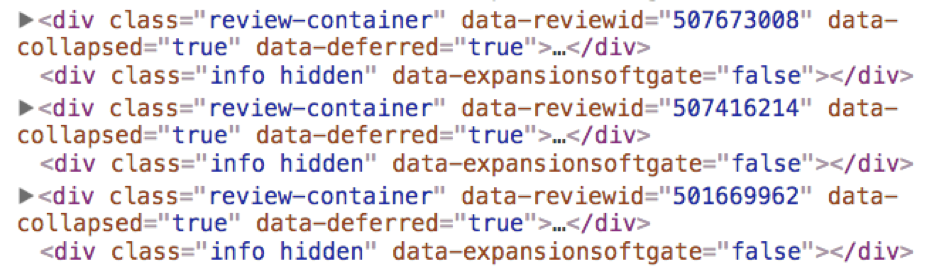
\includegraphics[width=\textwidth]{Bilder/reviewcontainer.png}
					\end{minipage}
					\centering
					\caption[Review Container]{Wiederholung der ‘review container' \cite{bib-reviewcontainer}}
					\label{pic-reviewcontainer}
				\end{figure}
				Mit dem erneuten Aufruf der Methode \textit{find\_all()} wird in einem container nach einem Link (\textit{<a>}-Tag) gesucht und gleichzeitig href auf \textit{‘True}‘ gesetzt. So stellt man sicher, dass nur Links mit href-Attribut ausgegeben werden. Bei diesem Link handelt es sich um den Teil der URL, der an die reguläre TripAdvisor Website angehängt werden muss, um die Bewertungsseite aufrufen zu können.
				\\
				Da jedoch nicht nur Informationen zur ersten gefunden Bewertung pro Seite, sondern zu allen Bewertungen extrahiert werden sollen, ist die Suchfunktion in eine weitere for-Schleife eingebunden. Diese loopt durch die vorher gespeicherte Liste \textit{review\_container}. So wird nicht nur der erste review container nach der Bewertungsseiten URL durchsucht sondern alle. Die Methode \textit{loop\_through\_review\_pages()} in Kombination mit der for Schleife über alle Bewertungsseiten ermöglicht nun die Bewertungslinks jeder einzelnen Bewertung auszulesen.
				\\
				\newline
				Diese neu ausgelesene URL wird jedes Mal an die Methode \textit{get\_single\_review\_data()} übergeben. Mit dieser können alle in Kapitel 3 definierten Daten zu den Bewertungen exrahiert werden.
	
	
	
			\subsection{Extraktion Bewertungensdaten}
			
				Auch hier muss zunächst wieder ein BeautifulSoup Object initalisiert werden, diesmal aber mit dem gespeicherten HTML-Code einer einzelnen Bewertungsseite (vgl. Programmcode 4.5).
				\\
				\begin{lstlisting} [caption={Initialisierung BeautifulSoup Object}\label{forpages}, captionpos=b, style=Arduino]
				def get_single_review_data(self,review_url):     
				source_code2 = requests.get(review_url)
				plain_text2 = source_code2.text
				soup = BeautifulSoup(plain_text2, "html.parser")
				\end{lstlisting}
	
	
			
		\section{Datenhaltung}
		%Einfach suche der Daten
			Eine Anforderung an das System besteht auch darin die gewonnenen Daten in einer Datenbank ablegen zu können. Zunächst wurden vom Product Owner die nötigen Ansprüche an die Datenbank bereitgestellt, nach der sich dann aus zwei Datenbanktypen eine vorteilhaftere herauskristallisieren konnte. 
			\\
			Da die gewonnen Rohdaten sich noch meist in einem encodierten Zustand befinden, müssen diese zunächst einen Bereinigungsprozess durchlaufen bevor sie leserlich in der Datenbank abgelegt werden können. Nicht nur das einfach Lesen der Daten sondern auch die Suche nach bestimmten Rechercheergebnissen soll möglichst intuitiv für den Nutzer ablaufen. Die Datenbankstruktur wurde daher Zusammen mit dem Auftraggeber abgestimmt und daraufhin die Architektur implementiert.
		
			\subsection{Definition der Datenbankanforderungen}
			
				Die vom Abnehmer vordefinierten Anforderungen an die Datenbank sind wie folgt:
				
				%Stichpunkte DB-Anforderungen															
				\begin{itemize}
					\item Integritätssicherung\\
					\begin{small}
						Daten werden auf Korrektheit (bereits während der Eingabe) überprüft und Fehlmanipulationen  verhindert 
					\end{small}
					
					\item Redundanzarmut\\
					\begin{small}
						es gibt keine ungeordnete Mehrfachspeicherung von Datenwerten
					\end{small}
								
					\item Datenunabhängigkeit\\
					\begin{small}
						die Datenbank kann ohne Server verwaltet und weiterentwickelt werden
					\end{small} 
					
					\item zentrale Kontrolle\\
					\begin{small}
						ein Administrator ist in der Lage, das gesamte System von einem Rechner aus zu verwalten
					\end{small}
				\end{itemize}
				
				
				\subsubsection{Vergleich: SQLLite und TinyDB}
				
					Im Folgenden werden zwei NoSQOL Datenbanktypen miteinander verglichen, die dem Entwicklerteam als am sinnvollsten erschienen.
					\\
					\underline{\textbf{TinyDB:}}
					\newline TinyDB ist eine leichtgewichtige dokumentenorientierte Datenbank, die für eine einfache Bedienung optimiert ist. Dabei ist sie in reinem Python geschrieben und hat keine externen Abhängigkeiten. Das Ziel sind kleine Apps, die von einer SQL-DB oder einem externen Datenbankserver entkoppelt funktionieren.
					\\					
					\underline{\textbf{SQLite:}}
					\newline SQLite ist eine gemeinfreie Programmbibliothek, die ein relationales Datenbanksystem enthält. Sie unterstützt einen Großteil der im SQL-92-Standard festgelegten SQL-Sprachbefehle. Die SQLite-Bibliothek lässt sich direkt in entsprechende Anwendungen integrieren, sodass keine weitere Server-Software benötigt wird. Dies ist der entscheidende Unterschied zu anderen Datenbanksystemen. Durch das Einbinden der Bibliothek wird die Anwendung um Datenbankfunktionen erweitert, ohne auf externe Softwarepakete angewiesen zu sein.
					\\
					\newline Der wesentliche Vorteil von TinyDB liegt darin, dass diese Datenbank bereits in Python geschrieben ist und sich somit ideal in unseren Source-Code integrieren lässt. Es entstehen dabei keine Inkonsistenzen oder fehlerhafte Bibliotheksaufrufe. Ein weiteres Plus ist die Möglichkeit das Dateiformat JSON als Datenbank zu verwenden. Dieses kann im Vergleich zur SQLite Datei in sehr vielen Anwendungen eingebunden und benutzt werden. Fortwährend ist man zu der Entscheidung gekommen, dass das Programmieren in SQL-Sprache in einem Python-Code zu Verwirrungen und unnötigen Programmier-Anforderungen beiträgt, was bei SQLite der Fall ist.
					\\
					Für das Projekt wurde sich einstimmig für die Verwendung von TinyDB als Datenbanksystem entschieden.
					
							
			\subsection{Datenbankstruktur}
			
				%Wie viele Tabellen, IDs, Verknüpfungen, Primärschlüssel
				Die extrahierten Daten können in grob vier Cluster eingeteilt werden, dabei bildet der erste Cluster die allgemeinen Daten des Restaurants, wie dessen Namen und Adresse. Den zweiten und dritten Cluster kann zusammenfassend als Benutzerdatenbank und Bewertungstext sehen. Der vierte Cluster bildet die Tabelle in der die Bilder abgespeichert werden, die zu einem jeweiligen Kommentar hinterlegt wurden.
				
				\subsubsection{Tabellen mit Spalten}
			
				\subsubsection{Zeichnung Zusammenhang?}


			\subsection{Daten bereinigen und integrieren}
				
				Meist sind die Daten auf den Webseiten bereits kodiert im UTF-8 Muster hinterlegt. UTF-8 (Abk. für 8-Bit UCS Transformation Format, wobei UCS wiederum Universal Character Set abkürzt) ist die am weitesten verbreitete Kodierung für Unicode-Zeichen. Es ist in den ersten 128 Zeichen (Indizes 0–127) deckungsgleich mit ASCII und eignet sich, mit in der Regel nur einem Byte Speicherbedarf, für Zeichen vieler westlicher Sprachen besonders für die Kodierung englischsprachiger Texte. \cite{bib-utf8} Die bei TripAdvisor angewendete Kodierung ist in dem Fall auch UTF-8 und muss neu decodiert werden, um die deutschen Umlaute korrekt anzeigen zu können.
				
				Nachdem die Rohdaten in Variablen abgelegt wurden, können diese in einer neuen Methode für den Reinigungsprozess weiterverwendet werden.
			
			
				
				
				
		\section{Benutzeroberfläche}
		
			\subsection{Wie die Umsetzung etc.}
			
			\subsection{Lösung mit URL}
	
	


	\chapter{Wurden Anforderungen erfüllt?}		
	
		\section{Ergebnisse}
		
	


	\chapter{Fazit und Ausblick}
	
		\section{Unsere Erfahrungen/Probleme (evtl. API)}

		\section{Wie sind wir damit klargekommen}


 
		
		Programmiersprache: Python
		hihii
				
			\begin{lstlisting} [caption={Registerprogrammierung der Expander}\label{code-i2c-1}, captionpos=b, style=Arduino]
			# -*- coding: utf-8 -*-
			import requests
			import os
			import unicodedata
			import validators
			import threading
			from tkinter import *
			from tkinter import messagebox
			from bs4 import BeautifulSoup
			from setuptools.package_index import HREF
			from tinydb import TinyDB,Query,where
			
			
			class Web_scraping:
			'''
			Created on 17.04.2018
			@author: anjawolf
			get_single_data: Data will be scraped from the Tripadvisors Website and stored in variables.
			'''
			def get_single_data(self,url):
			source_code = requests.get(url)
			plain_text = source_code.text
			soup = BeautifulSoup(plain_text, "html.parser")
			
			for self.name in soup.find('h1', {'class': 'heading_title'}):
			print("Name:" + self.name.string)
			
			for self.rating_amount in soup.find('span', {'property': 'count'}):
			print("Anzahl Bewertungen:" + self.rating_amount.string)
			
			for self.popularity in soup.find_all('span', {'class': 'header_popularity popIndexValidation'}):
			print("Popularitaet:" + self.popularity.text)
			
			for self.price_level in soup.find('span', {'class': 'header_tags rating_and_popularity'}):
			print("Preis Level:" + self.price_level.string)
			
			for self.cuisine in soup.find_all('span', {'class': 'header_links rating_and_popularity'}):
			print('Kueche:' + self.cuisine.text)
			
			for self.contact_details in soup.find('div', {'class': 'blRow'}):
			print('Kontaktdaten:' + self.contact_details.text)
			
			for self.address in soup.find('span', {'class': 'street-address'}):
			print("Strasse:" + self.address.string)
			
			for self.locality in soup.find('span', {'class': 'locality'}):
			print("PLZ:" + self.locality.string)
			
			for self.phonenumber in soup.find_all('div', {'class': 'blEntry phone'}):
			print("Telefonnummer:" + self.phonenumber.text)
			
						     
			\end{lstlisting}
	
	
	
	
%						    	Hinzufügen relevanter Verzeichnisse
%   									Abbildungsverzeichnis
	\clearpage
	\addcontentsline{toc}{chapter}{Abbildungsverzeichnis}
	\listoffigures
	
	
	
%   									Programmcodeverzeichnis	
	\clearpage
	%Erneute Bennenung für das Verzeichnis 
	\addcontentsline{toc}{chapter}{Programmcodeverzeichnis}
	\renewcommand{\lstlistingname}{Programmcodeverzeichnis}
	\lstlistoflistings
	\renewcommand{\lstlistlistingname}{\lstlistingname}
	
	
	
%   									Abkürzungsverzeichnis	
	\chapter*{Abkürzungsverzeichnis}
		\vspace{1.0cm}
		\begin{acronym}[SEPSEP]
			\acro{oem}[OEM]{Original Equipment Manufacturer}
			\acro{bob}[BOB]{Breakout-Box}
			\acro{can}[CAN]{Controller Area Network}
			\acro{lin}[LIN]{Local Interconnect Network}
			\acro{obd}[OBD]{On-Board-Diagnose}	
			\acro{sda}[SDA]{Serial Data Line}
			\acro{scl}[SCL]{Serial Clock Line}
			\acro{gui}[GUI]{Graphical User Interface}
			\acro{pdf}[PDF]{Portable Document Format}
			%\acro{SD}[SD]{Secure Digital Memory Card}
			%\acro{pc}[PC]{Personal Computer}
			%\acro{USB}[USB]{Universal Serial Bus}
		\end{acronym}
		\addcontentsline{toc}{chapter}{Abkürzungsverzeichnis}
	
	
	
%   									Literaturverzeichnis	
	\clearpage
	\addcontentsline{toc}{chapter}{Literaturverzeichnis}
	\begin{thebibliography}{9} 
		\vspace{1.0cm}
		%Internetrecherche 
		
		\bibitem{bib-atomfeed} Atom Feed\\ Ryte Wiki: Atom Feed, \newline \url{https://de.ryte.com/wiki/Atom_Feed}, aufgerufen am \today
					
		\bibitem{bib-deepweb} Deep Web\\ Advidera: Deep Web, \newline \url{https://www.advidera.com/glossar/deep-web}, aufgerufen am \today	
		
		\bibitem{bib-utf8} Kodierung in UTF-8\\ UTF-8, \newline \url{https://de.wikipedia.org/wiki/UTF-8}, aufgerufen am \today
		
		\bibitem{bib-daten} Definition von Datenarten zur konsistenten Kommunikation im Unternehmen\\ Piro A., Gebauer M. Hrsg: \glqq Vieweg und Teubner in Daten- und Informationsqualität.\grqq, S.143 - 156
		
		\bibitem{bib-webpython} Web scraping with Python: collecting data from the modern web\\ Mitchel, R. Hrsg: \O'Reilly Media, Inc.
		
		\bibitem{bib-bs4} Beautiful Soup Documentation, \newline \url{http://www.crummy.com/software/BeautifulSoup/bs4/doc/} aufgerufen am \today
		
		\bibitem{bib-reviewcontainer} Screenshot Review Container,\newline \url{https://www.tripadvisor.de/Restaurant_Review-g504000-d720608-Reviews-Star_Inn-Harome_North_Yorkshire_England.html}, aufgerufen am \today
		
		%Buchrecherche
		%\bibitem{bib-handb} Kraftfahrzeugtechnik \\ Hans-Hermann Braess, Ulrich Seiffert Hrsg: \glqq Vieweg Handbuch Kraftfahrzeugtechnik\grqq, Springer-Vieweg-Verlag, S. 5, 7. Auflage 2013
	\end{thebibliography}
	
	
	
%   									Selbstständigkeitserklärung
	\newpage
	\setstretch{1.5}
	\chapter*{Eidesstattliche Erklärung}
		%\vspace{1.5\textheight}
		Hiermit erklären wir, Johannes Knippel, Anja Wolf, Johanna Sickendiek und Skanny, dass wir die vorliegende Arbeit mit dem Titel \textit{Extraktion unstrukturierter Daten und Integration in eine Datenbank am Beispiel TripAdvisor} selbstständig verfasst, noch nicht anderweitig für Prüfungszwecke vorgelegt, keine anderen als die angegebenen Quellen oder Hilfsmittel benützt sowie wörtliche und sinngemäße Zitate als solche gekennzeichnet haben.
		\vspace{15mm}
		\\
		\\
		\begin{flushleft}
			\begin{tabular}[H]{ll}
				
				München, den \parbox{5,5cm}{\today}  	& 	\parbox{6cm}{\hrule\medskip \textit{Unterschrift}}\\[2cm]
													  	& 	\parbox{6cm}{\hrule\medskip \textit{Unterschrift}}\\[2cm]
													  	& 	\parbox{6cm}{\hrule\medskip \textit{Unterschrift}}\\[2cm]
													  	& 	\parbox{6cm}{\hrule\medskip \textit{Unterschrift}}\\[2cm]
			\end{tabular}
		\end{flushleft}
		\addcontentsline{toc}{chapter}{Eidesstattliche Erklärung}


\end{document}
%The End
%Johannes Knippel